\documentclass{standalone}
\usepackage{tikz}
\usetikzlibrary{patterns, positioning}


\begin{document}
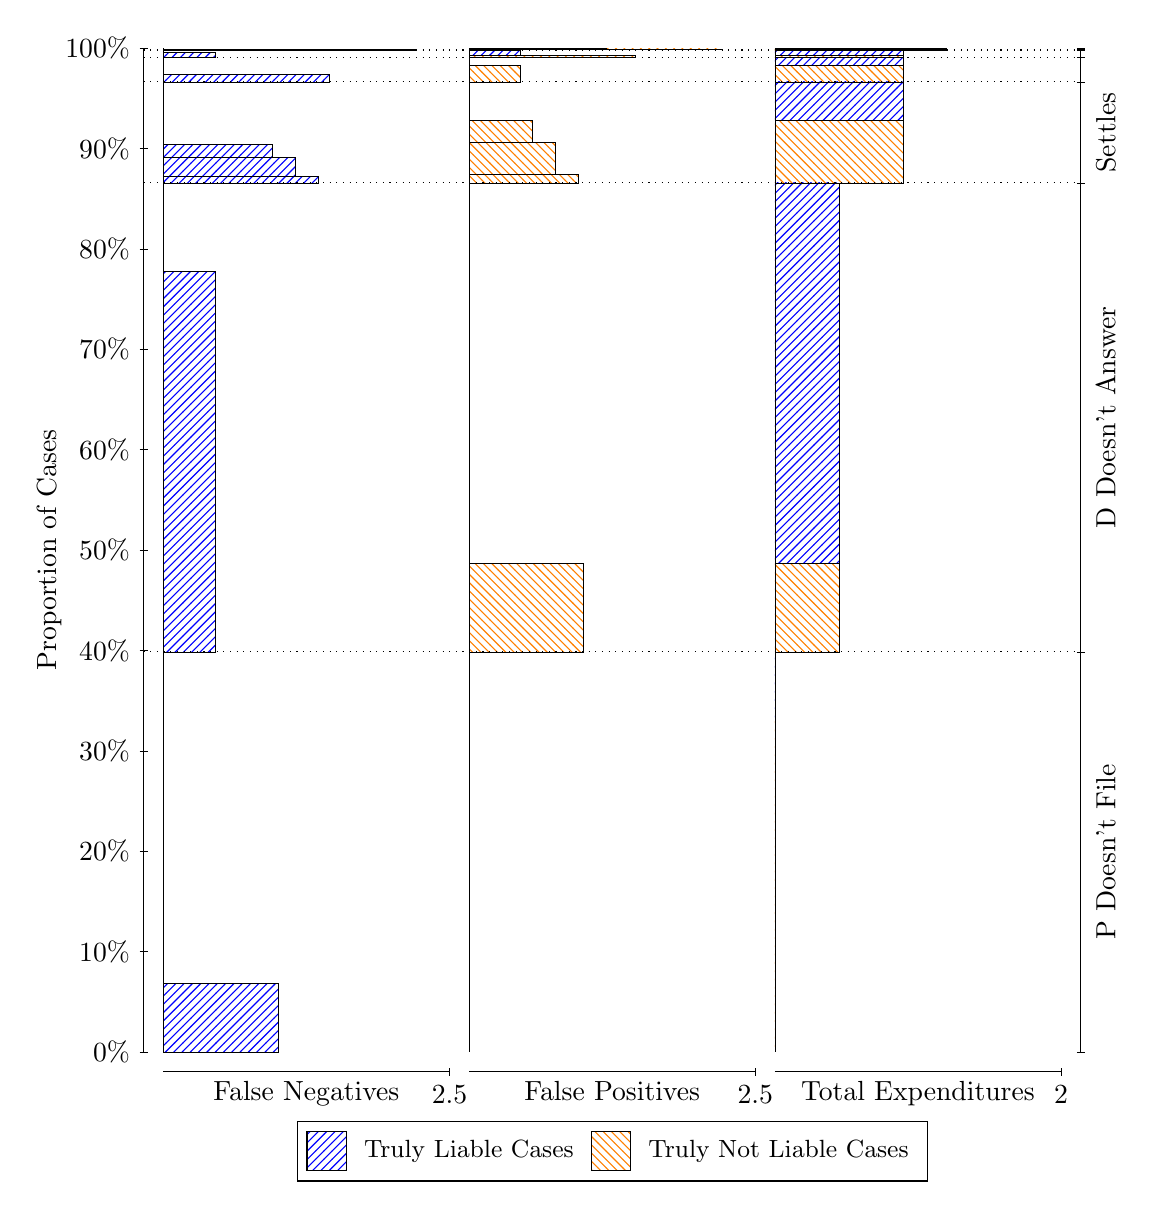
\begin{tikzpicture}
\draw[black, very thin] (1.5,1.75) -- (1.5,14.5);
\node[rotate=90, text=black, anchor=center] at (0.3, 8.125) {Proportion of Cases};
\draw[black, very thin] (1.45,1.75) -- (1.55,1.75);
\node[text=black, anchor=east] at (1.45, 1.75) {0\%};
\draw[black, very thin] (1.45,3.025) -- (1.55,3.025);
\node[text=black, anchor=east] at (1.45, 3.025) {10\%};
\draw[black, very thin] (1.45,4.3) -- (1.55,4.3);
\node[text=black, anchor=east] at (1.45, 4.3) {20\%};
\draw[black, very thin] (1.45,5.575) -- (1.55,5.575);
\node[text=black, anchor=east] at (1.45, 5.575) {30\%};
\draw[black, very thin] (1.45,6.85) -- (1.55,6.85);
\node[text=black, anchor=east] at (1.45, 6.85) {40\%};
\draw[black, very thin] (1.45,8.125) -- (1.55,8.125);
\node[text=black, anchor=east] at (1.45, 8.125) {50\%};
\draw[black, very thin] (1.45,9.4) -- (1.55,9.4);
\node[text=black, anchor=east] at (1.45, 9.4) {60\%};
\draw[black, very thin] (1.45,10.675) -- (1.55,10.675);
\node[text=black, anchor=east] at (1.45, 10.675) {70\%};
\draw[black, very thin] (1.45,11.95) -- (1.55,11.95);
\node[text=black, anchor=east] at (1.45, 11.95) {80\%};
\draw[black, very thin] (1.45,13.225) -- (1.55,13.225);
\node[text=black, anchor=east] at (1.45, 13.225) {90\%};
\draw[black, very thin] (1.45,14.5) -- (1.55,14.5);
\node[text=black, anchor=east] at (1.45, 14.5) {100\%};

\draw[black, very thin] (13.4,1.75) -- (13.4,14.5);
\draw[black, very thin] (13.35,1.75) -- (13.45,1.75);
\node[anchor=west] at (13.35, 1.75) {};
\draw[black, very thin] (13.35,6.8304) -- (13.45,6.8304);
\node[anchor=west] at (13.35, 6.8304) {};
\draw[black, very thin] (13.35,12.787) -- (13.45,12.787);
\node[anchor=west] at (13.35, 12.787) {};
\draw[black, very thin] (13.35,14.07) -- (13.45,14.07);
\node[anchor=west] at (13.35, 14.07) {};
\draw[black, very thin] (13.35,14.377) -- (13.45,14.377);
\node[anchor=west] at (13.35, 14.377) {};
\draw[black, very thin] (13.35,14.473) -- (13.45,14.473);
\node[anchor=west] at (13.35, 14.473) {};
\draw[black, very thin] (13.35,14.484) -- (13.45,14.484);
\node[anchor=west] at (13.35, 14.484) {};
\draw[black, very thin] (13.35,14.5) -- (13.45,14.5);
\node[anchor=west] at (13.35, 14.5) {};

\draw[black, very thin, pattern color=blue, pattern=north east lines] (1.75,1.75) rectangle (3.2033,2.6245);
\draw[black, very thin, pattern color=orange, pattern=north west lines] (1.75,2.6245) rectangle (1.75,6.8304);
\draw[black, very thin, pattern color=blue, pattern=north east lines] (1.75,6.8304) rectangle (2.404,11.663);
\draw[black, very thin, pattern color=orange, pattern=north west lines] (1.75,11.663) rectangle (1.75,12.787);
\draw[black, very thin, pattern color=blue, pattern=north east lines] (1.75,12.787) rectangle (3.712,12.867);
\draw[black, very thin, pattern color=blue, pattern=north east lines] (1.75,12.867) rectangle (3.4213,13.108);
\draw[black, very thin, pattern color=blue, pattern=north east lines] (1.75,13.108) rectangle (3.1307,13.274);
\draw[black, very thin, pattern color=orange, pattern=north west lines] (1.75,13.274) rectangle (1.75,14.07);
\draw[black, very thin, pattern color=blue, pattern=north east lines] (1.75,14.07) rectangle (3.8573,14.163);
\draw[black, very thin, pattern color=orange, pattern=north west lines] (1.75,14.163) rectangle (1.75,14.377);
\draw[black, very thin, pattern color=blue, pattern=north east lines] (1.75,14.377) rectangle (2.404,14.449);
\draw[black, very thin, pattern color=orange, pattern=north west lines] (1.75,14.449) rectangle (1.75,14.473);
\draw[black, very thin, pattern color=blue, pattern=north east lines] (1.75,14.473) rectangle (4.9473,14.478);
\draw[black, very thin, pattern color=orange, pattern=north west lines] (1.75,14.478) rectangle (1.75,14.484);
\draw[black, very thin, pattern color=orange, pattern=north west lines] (1.75,14.484) rectangle (1.75,14.489);
\draw[black, very thin, pattern color=blue, pattern=north east lines] (1.75,14.489) rectangle (1.75,14.5);
\draw[black, very thin, pattern color=orange, pattern=north west lines] (5.6333,1.75) rectangle (5.6333,5.9559);
\draw[black, very thin, pattern color=blue, pattern=north east lines] (5.6333,5.9559) rectangle (5.6333,6.8304);
\draw[black, very thin, pattern color=orange, pattern=north west lines] (5.6333,6.8304) rectangle (7.0867,7.9546);
\draw[black, very thin, pattern color=blue, pattern=north east lines] (5.6333,7.9546) rectangle (5.6333,12.787);
\draw[black, very thin, pattern color=orange, pattern=north west lines] (5.6333,12.787) rectangle (7.014,12.899);
\draw[black, very thin, pattern color=orange, pattern=north west lines] (5.6333,12.899) rectangle (6.7233,13.306);
\draw[black, very thin, pattern color=orange, pattern=north west lines] (5.6333,13.306) rectangle (6.4327,13.583);
\draw[black, very thin, pattern color=blue, pattern=north east lines] (5.6333,13.583) rectangle (5.6333,14.07);
\draw[black, very thin, pattern color=orange, pattern=north west lines] (5.6333,14.07) rectangle (6.2873,14.284);
\draw[black, very thin, pattern color=blue, pattern=north east lines] (5.6333,14.284) rectangle (5.6333,14.377);
\draw[black, very thin, pattern color=orange, pattern=north west lines] (5.6333,14.377) rectangle (7.7407,14.402);
\draw[black, very thin, pattern color=blue, pattern=north east lines] (5.6333,14.402) rectangle (6.2873,14.473);
\draw[black, very thin, pattern color=orange, pattern=north west lines] (5.6333,14.473) rectangle (5.6333,14.479);
\draw[black, very thin, pattern color=blue, pattern=north east lines] (5.6333,14.479) rectangle (5.6333,14.484);
\draw[black, very thin, pattern color=orange, pattern=north west lines] (5.6333,14.484) rectangle (8.8307,14.489);
\draw[black, very thin, pattern color=blue, pattern=north east lines] (5.6333,14.489) rectangle (7.3773,14.5);
\draw[black, very thin, pattern color=orange, pattern=north west lines] (9.5167,1.75) rectangle (9.5167,5.9559);
\draw[black, very thin, pattern color=blue, pattern=north east lines] (9.5167,5.9559) rectangle (9.5167,6.8304);
\draw[black, very thin, pattern color=orange, pattern=north west lines] (9.5167,6.8304) rectangle (10.334,7.9546);
\draw[black, very thin, pattern color=blue, pattern=north east lines] (9.5167,7.9546) rectangle (10.334,12.787);
\draw[black, very thin, pattern color=orange, pattern=north west lines] (9.5167,12.787) rectangle (11.152,13.583);
\draw[black, very thin, pattern color=blue, pattern=north east lines] (9.5167,13.583) rectangle (11.152,14.07);
\draw[black, very thin, pattern color=orange, pattern=north west lines] (9.5167,14.07) rectangle (11.152,14.284);
\draw[black, very thin, pattern color=blue, pattern=north east lines] (9.5167,14.284) rectangle (11.152,14.377);
\draw[black, very thin, pattern color=orange, pattern=north west lines] (9.5167,14.377) rectangle (11.152,14.402);
\draw[black, very thin, pattern color=blue, pattern=north east lines] (9.5167,14.402) rectangle (11.152,14.473);
\draw[black, very thin, pattern color=orange, pattern=north west lines] (9.5167,14.473) rectangle (11.697,14.479);
\draw[black, very thin, pattern color=blue, pattern=north east lines] (9.5167,14.479) rectangle (11.697,14.484);
\draw[black, very thin, pattern color=orange, pattern=north west lines] (9.5167,14.484) rectangle (11.697,14.489);
\draw[black, very thin, pattern color=blue, pattern=north east lines] (9.5167,14.489) rectangle (11.697,14.5);
\draw[black, dotted] (1.5,6.8304) -- (13.4,6.8304);
\draw[black, dotted] (1.5,12.787) -- (13.4,12.787);
\draw[black, dotted] (1.5,14.07) -- (13.4,14.07);
\draw[black, dotted] (1.5,14.377) -- (13.4,14.377);
\draw[black, dotted] (1.5,14.473) -- (13.4,14.473);
\draw[black, dotted] (1.5,14.484) -- (13.4,14.484);
\draw[black, very thin] (1.75,1.5) -- (5.3833,1.5);
\node[text=black, anchor=north] at (3.5667, 1.5) {False Negatives};
\draw[black, very thin] (5.3833,1.45) -- (5.3833,1.55);
\node[text=black, anchor=north] at (5.3833, 1.45) {2.5};

\draw[black, very thin] (5.6333,1.5) -- (9.2667,1.5);
\node[text=black, anchor=north] at (7.45, 1.5) {False Positives};
\draw[black, very thin] (9.2667,1.45) -- (9.2667,1.55);
\node[text=black, anchor=north] at (9.2667, 1.45) {2.5};

\draw[black, very thin] (9.5167,1.5) -- (13.15,1.5);
\node[text=black, anchor=north] at (11.333, 1.5) {Total Expenditures};
\draw[black, very thin] (13.15,1.45) -- (13.15,1.55);
\node[text=black, anchor=north] at (13.15, 1.45) {2};

\node[text=black, centered, rotate=90] at (13.72, 4.2902) {P Doesn't File};
\node[text=black, centered, rotate=90] at (13.72, 9.8088) {D Doesn't Answer};
\node[text=black, centered, rotate=90] at (13.72, 13.429) {Settles};





\draw (7.449999999999999,1.5) node[draw=none] (baseCoordinate) {};
\begin{scope}[align=center]
        \matrix[scale=0.5, draw=black, below=0.5cm of baseCoordinate, nodes={draw}, column sep=0.1cm]{
            \node[rectangle, draw, minimum width=0.5cm, minimum height=0.5cm, pattern color=blue, pattern=north east lines] {}; &
            \node[draw=none, font=\small, text=black] (B) {Truly Liable Cases}; &
            \node[rectangle, draw, minimum width=0.5cm, minimum height=0.5cm, pattern color=orange, pattern=north west lines] {}; &
            \node[draw=none, font=\small, text=black] (B) {Truly Not Liable Cases}; \\
            };
\end{scope}

\end{tikzpicture}
\end{document}